\setAuthor{}
\setRound{lõppvoor}
\setYear{2020}
\setNumber{G 8}
\setDifficulty{8}
\setTopic{TODO}

\prob{Optiline seade}
\begin{wrapfigure}{r}{0.35\textwidth}
  \vspace{-25pt}
  \begin{center}
  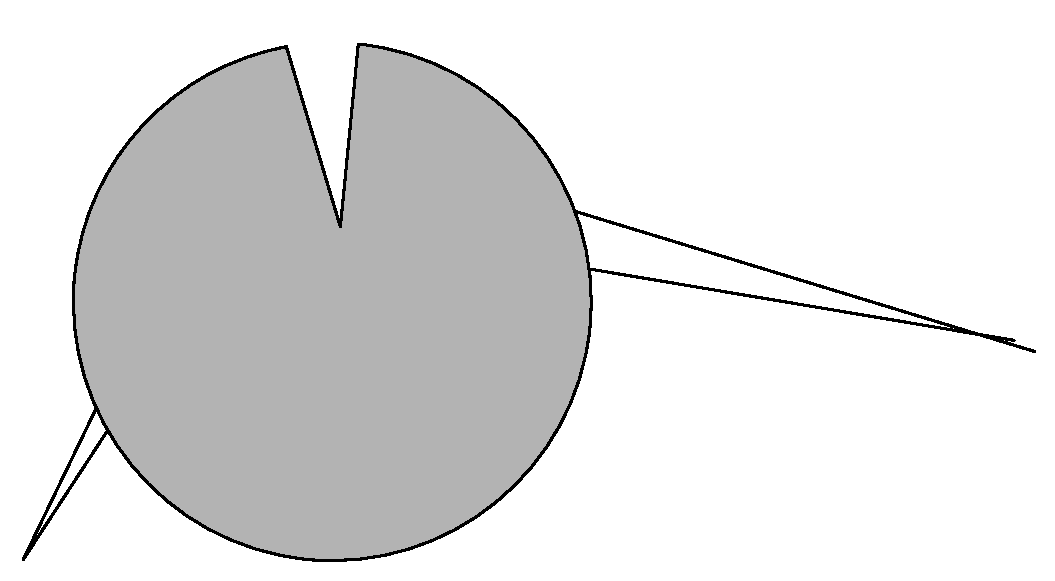
\includegraphics[scale=0.25]{2020-v3g-08-yl.pdf}
  \end{center}
  \vspace{-25pt}
\end{wrapfigure}
Kiilukujulise sisselõikega silindri sees on kaks üksteisega paralleelset peeglit,
mis on paralleelsed ka silindri teljega. Valguskiired saavad silindrisse siseneda
ja sealt väljuda läbi silindri seintes olevate aukude. Silinder on seest õõnes
ning selle seinad on mittepeegeldavad. Joonisel on kujutatud
silinder pealtvaates koos kahe silindrisse siseneva ning peale peegeldusi sealt
väljuva kiirega. Rekonstrueerige peeglite asukohad ning kiirte käik (leidke
vähemalt üks võimalik lahendus). Lahendus esitage lisalehel.


\hint

\solu
\begin{figure}[h]
\centering
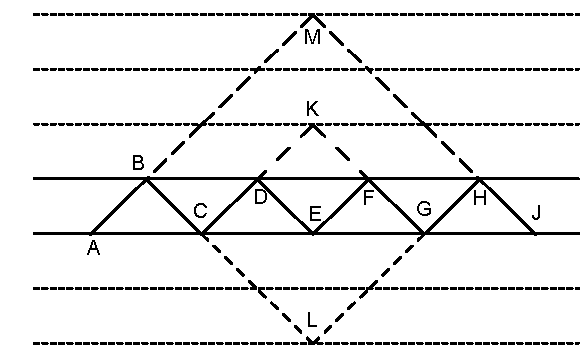
\includegraphics[width=0.5\linewidth]{2020-v3g-08-yl1.pdf}\par
Joonis 1
\end{figure}
Kõigepealt vaatleme kiirte käiku kahe paralleelse peegli vahel joonisel 1. Kui peegeldame sik-sakilisest kiirest jupi $DEF$ ülemises peeglis, saame jupi $DKF$, mis koos lõikudega $CD$ ning $FG$ moodustab juba vähemate sik-sakkidega jupi $CKG$. Peegeldades juppi $CKG$  alumises peeglis saame jupi $CLG$ ning korrates peegeldamist veel ühe korra saame tervest sik-sakilisest teekonnast $ABCDEFGHJ$ teekonna $AMJ$, mida võib vaadelda kui kiire $AB$ peegeldust alumise peegli kujutise-kujutise-kujutises. Niisiis, kui joonistame peeglite kujutised, kujutise-kujutised jne, näeme, et sisenevad kiired justkui peegelduksid peeglite kujutises või kujutise-kujutises või kujutise-kujutise-kujutises jne. Algsel joonisel toodud kiirte põhjal saame taastada kaks sellist kujutist, kujutise-kujutist või kujutise-kujutise-kujutist  või jne. N-järku kujutiste seeria moodustab paralleelsete sirgete rivi; tegelikud peeglid peavad olema ühed neist. Kui me joonistame sisendkiiri väljundkiirteks peegeldavate  sirgetega (mis on leitavad kiirte pikenduste lõikepunkte läbivate nurgapoolitajate ristsirgetena) paraleelsete ja võrdsetel vahekaugustel asuvate sirgete rivi, siis peavad tegelikud peeglid asuma kahel naabersirgel.

\begin{figure}[h]
\centering
  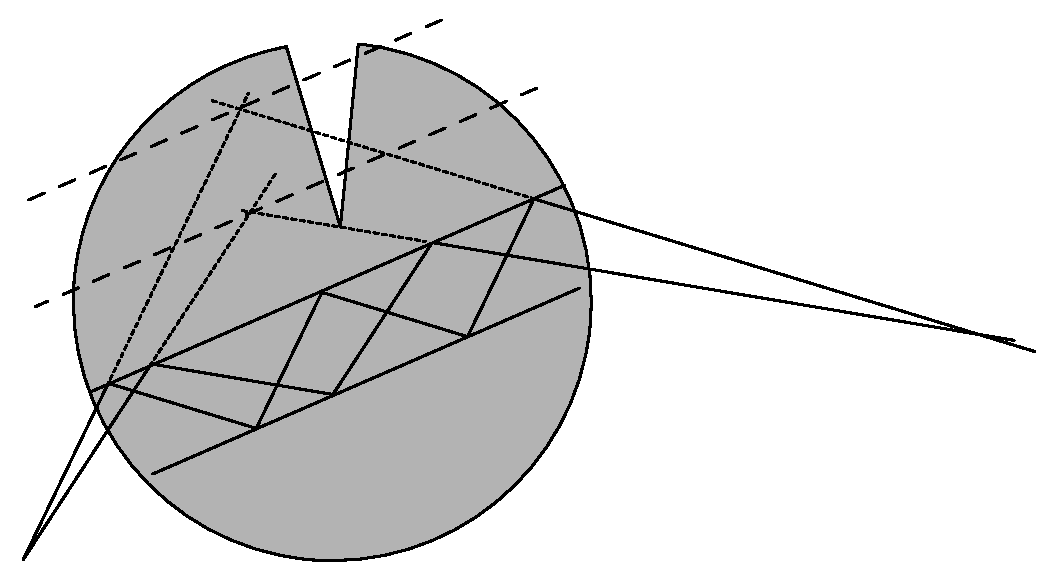
\includegraphics[width=0.4\textwidth]{2020-v3g-08-yl2.pdf}
  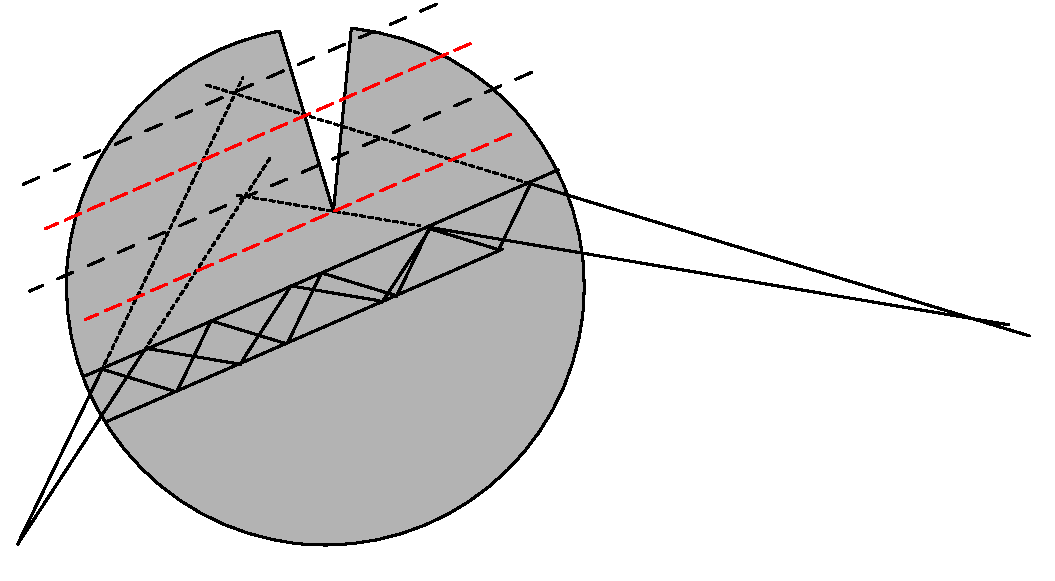
\includegraphics[width=0.4\textwidth]{2020-v3g-08-yl3.pdf}
  \par
  \begin{tabular}{p{0.5\linewidth}p{0.5\linewidth}}
  \hfil Joonis 2. & \hfil Joonis 3. \\
  \end{tabular}
\end{figure}

Joonisel 2 on näha, et lihtsaimal juhul välistab sisselõige peeglite asukoha kõigis peale kahe alumise (veel madalamad asukohad pole võimalikud seetõttu, et sisendkiired ei saa nende vahele siseneda). Põhimõtteliselt on võimalik ka joonisel 3 toodud variant.
\probend